\section{System Model and Receipt-Gated Handoff}
Figure~\ref{fig:control_architecture} shows the shared architecture. Event
producers send messages through ingest services to durable subscription queues.
Subscriber Pods deliver them to clients over persistent connections. The
transport load balancer assigns new sockets; the client selects whether to
promote its retained probe. Additional component descriptions are provided in
the Online Supplementary Material.
\subsection{Retained-Probe Acquisition and Receipt-Gated Handoff}
\label{sec:probe_handoff}

Figure~\ref{fig:control_architecture} makes the selected-Pod mechanism
explicit. The client does not choose a Pod name and then attempt to bypass the
Kubernetes Service. It opens an authenticated, statistics-only probe through
the same transport load balancer used by ordinary connections. The load
balancer selects one ready subscriber Pod when that TCP/WebSocket connection is
established, after which the socket remains endpoint-bound to that Pod. The
STOMP implementation identifies the authenticated session and its Pod in
telemetry. A probe initially has no subscription bindings and does not fetch
events. Promotion changes the role of that existing session; it does not
create a second connection whose load-balanced destination might differ.

The selector evaluates a candidate that is already connected. Fresh and
sufficiently complete telemetry, a distinct source and target Pod, capacity,
cooldown, and handoff checks determine whether migration is admissible. The
DQL selector also applies its action-value hysteresis test. A rejected or
unselected probe remains statistics-only until refreshed or recycled. Thus,
probing does not imply migration, and the client never moves an established
TCP socket between endpoints. It replaces one delivery socket with the
already-connected probe and reassociates the source subscriptions.
In Figure~\ref{fig:control_architecture}, $c_p$ labels the retained probe,
whose endpoint is $i_u^{\mathrm{probe}}(t)$. The source and existing target Pod indices
are $i_h=i_{u,c_h}(t)$ and $i_l=i_{u,c_l}(t)$. Thus $i_h$ and $i_l$ identify
Pods, while $P_i(t)$ denotes a pressure score.

Queued events remain in the same durable subscription queues $Q_{u,k}(t)$.
The client retains each subscription identifier, listener, message permits,
and negative-acknowledgement visibility setting. For the selected subscription
set $\mathcal{K}_{\mathrm{move}}$, the executed protocol is:
\begin{enumerate}
	\item Create each target binding in \emph{standby}, waiting for its STOMP
	receipt. The first subscription request carries the probe-promotion flag.
	The server checks the authenticated session and its active-connection cap,
	then changes the probe's role. Standby bindings do not deliver events.
	The source remains active while these target bindings are prepared.
	\item After all standby receipts, add the promoted socket to the client
	pool and clear its probe role. Send a receipt-gated quiesce request for each
	source binding. Quiescence stops new delivery while existing in-flight
	messages remain on the source acknowledgement path.
	\item Record a barrier timestamp after the quiesce requests. Wait for a
	newer source telemetry frame that reports every selected subscription as
	quiesced with zero in-flight messages. A zero from an older frame cannot
	satisfy the barrier. Drain time is observed, not estimated from $H_i$.
	\item Activate the target bindings one at a time, waiting for their
	receipts. The source remains quiesced during this phase.
	\item Unsubscribe the source bindings with receipt checks. After all
	selected bindings are detached, remove and disconnect the old socket for
	a full-connection migration. Replenish the subscription-free probe
	asynchronously. Unselected active sockets remain connected.
\end{enumerate}

Let $s_b$ be the barrier timestamp, $s_f$ the timestamp of a received source
frame, and $I_{c_h,k}(s_f)$ its reported in-flight count. The target-activation
precondition is
\begin{equation}
	 s_f\geq s_b\quad\land\quad
	 \bigwedge_{k\in\mathcal{K}_{\mathrm{move}}}
	 \left[\operatorname{state}_{c_h,k}(s_f)=\mathrm{quiesced}
	 \land I_{c_h,k}(s_f)=0\right].
	\label{eq:handoff_barrier}
\end{equation}
This precondition describes the implemented planned handoff, assuming timely,
accurate telemetry and servers that honor quiescence. It is not a distributed
ownership lease or an epoch-fencing guarantee during partitions. On an
exception, the client attempts to quiesce and close the target before restoring
the source; unsuccessful cleanup is logged rather than counted as a completed
handoff. The protocol uses authenticated session state and receipts, not a
separate signed promotion token or an atomic cross-Pod ownership commit.
Receipt completion records server acknowledgement of the corresponding
operation; it is not by itself proof of an end-to-end exactly-once event census.
The delivery model remains unordered and permits redelivery after an
unconfirmed acknowledgement. The live results report observed deliveries,
ACK receipts, and unresolved records separately.

\afterpage{
\begin{landscape}
\begin{figure}[p]
	\centering
	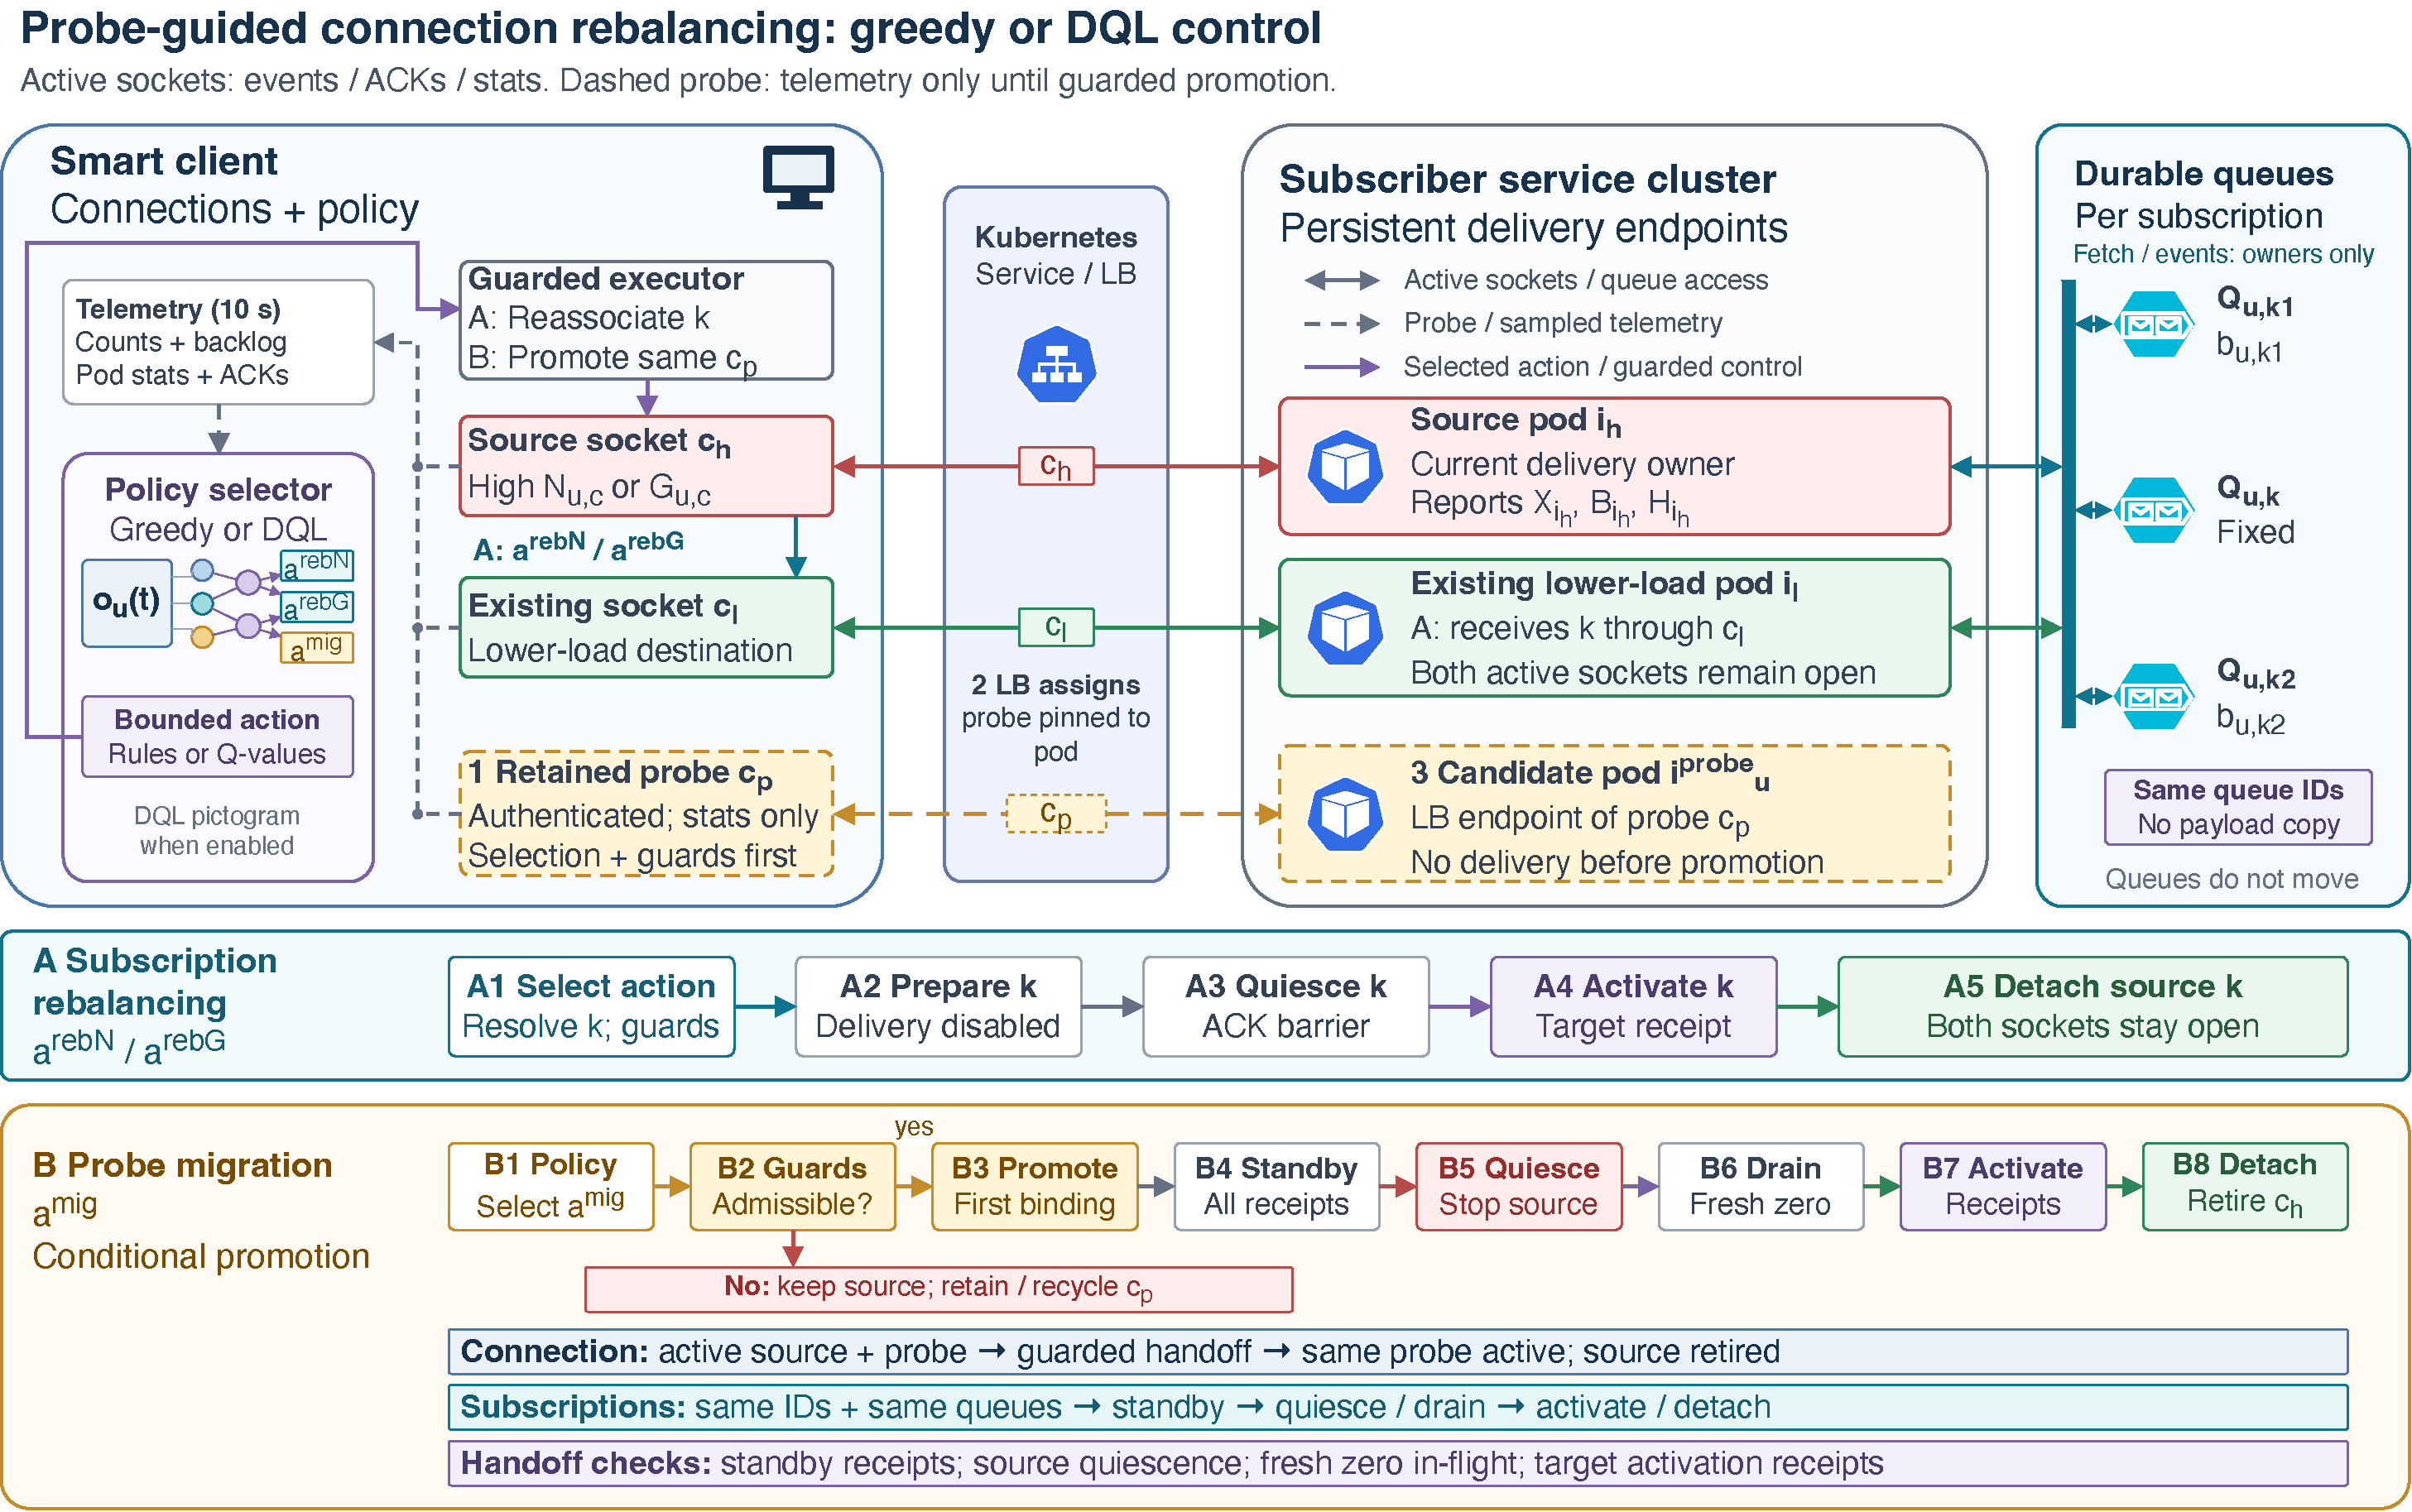
\includegraphics[width=\linewidth,height=0.83\textwidth,keepaspectratio]{figures/control-architecture-original-style.pdf}
	\caption{Shared probe-guided architecture with greedy or DQL selection. Path A rebalances subscriptions between existing sockets. Path B promotes the retained probe through its first standby binding, waits for all standby receipts, quiesces and drains the source, activates the target, detaches the source bindings, and retires the old socket. Unselected sockets and durable queues remain in place. The DQL pictogram denotes the optional learned selector, not an additional handoff service.}
	\Description{Two-path architecture with clients, subscriber Pods, and durable queues. Active and probe telemetry feed a greedy or DQL selector and a shared guarded executor. The selected probe keeps its load-balanced endpoint. Standby receipts, source quiescence, fresh zero-in-flight telemetry, activation receipts, and source detachment govern handoff. No ownership registry or epoch-commit service is shown.}
	\label{fig:control_architecture}
\end{figure}
\end{landscape}
}
